\documentclass{xduugtrans}
\graphicspath{{figures}}
% TODO: 封面需要修改成与翻译任务相匹配的封面
\xdusetup{
    style = {
        bib-backend = bibtex,
        before-skip = {24pt, 18pt, 12pt, 12pt, 12pt, 12pt}, % 标题前间距
        after-skip = {18pt, 12pt, 12pt, 12pt, 12pt, 12pt}, % 标题后间距
    },
    info = {
        title = {Hawk: 基于密码学和 \\ 智能合约隐私保护的区块链模型},
        department = {计算机科学与技术学院},
        major = {计算机科学与技术},
        author = {石学舟},
        supervisor = {张南},
        % supervisor-department = {王五},
        % supervisor-enterprise = {赵六},
        % supervisor-school = {刘七},
        class-id = {1803013},
        student-id = {18010500076},
        abstract = {abstract-zh.tex},
        abstract* = {abstract-en.tex},
        keywords = {Hawk,区块链},
        keywords* = {Hawk,blockchain},
        acknowledgements = {acknowledgements.tex}
    }
}
\begin{document}
\frontmatter
\mainmatter
\chapter{概述}
比特币\cite{ref48} 和代币\cite{ref20}等去中心化加密货币迅速普及,并经常被引用作为对我们未来的一瞥\cite{ref5}。这些新兴的加密货币系统建立在一种新颖的区块链技术之上,其中矿工运行分布式共识,其安全性得到保证,如果没有对手使用大部分计算(或其他形式的)资源。术语“区块链”和“矿工”因此经常互换使用。

像比特币这样的区块链不仅在数据流上达成共识,而且在涉及这些数据的计算上也达成共识。具体来说,在比特币中,数据包括用户提出的转账交易,计算涉及交易验证和更新称为未使用交易输出集的数据结构,不准确地说,它跟踪用户的账户余额。新兴的加密货币系统,如以太坊\cite{ref57}采用了在区块链上运行任意用户定义程序的想法,从而创建了一个富有表现力的去中心化智能合约系统。

在本文中,我们考虑了各方与此类区块链交互的智能合约协议。假设去中心化共识协议是安全的,那么区块链可以被认为是一个概念方(实际上是去中心化的),可以信任其正确性和可用性,但不能信任隐私。这样的区块链为分布式协议的设计提供了强大的抽象。

区块链自然地体现了一个离散的时间概念,即每当挖掘一个新区块时,时钟就会递增,这一事实进一步增强了区块链的表达能力。这种可信时钟的存在对于在协议中实现财务公平至关重要。特别是,恶意的合同方可能会过早地中止协议以避免财务支付。然而,有了一个可信的时钟,可以使用超时来使这种中止明显,这样区块链就可以通过将他们的抵押存款重新分配给诚实的非中止的一方来对中止方进行经济上的惩罚。这使得密码学的区块链模型比没有区块链的传统模型更强大,在传统模型中,当大多数各方都可能腐败时,人们早就知道公平是不可能的\cite{ref8}\cite{ref17}\cite{ref24}。总之,区块链允许相互不知情的各方在没有中央信任中介的情况下安全地进行交易,并避免高昂的法律和交易成本。

尽管区块链和智能合约具有优秀的表现力和力量,这些技术的当前形式缺乏交易隐私。智能合约中采取的整个行动序列通过网络传播或记录在区块链上,因此是公开可见的。尽管各方可以创建新的假名公钥来增加他们的匿名性,但每个(假名)公钥的所有交易和余额的价值都是公开可见的。此外,最近的工作还通过分析加密货币的事务图结构来证实了去匿名化攻击(的可行性)\cite{ref42}\cite{ref52}。

我们强调,缺乏隐私是广泛采用去中心化智能合约的主要障碍,因为许多个人和组织认为金融交易(例如保险合约或股票交易)是高度机密的。尽管在设计诸如 Zerocash \cite{ref11} 和其他几个 \cite{ref26}\cite{ref43}\cite{ref54} 等保护隐私的加密货币方面取得了进展,但这些系统放弃了可编程性,并且事先并不清楚如何在不暴露交易的情况下实现可编程性并以明文形式向矿工提供数据。

\section{Hawk 简介}
我们提出了 \textbf{Hawk},一个用于构建保护隐私的智能合约的框架。 使用 \textbf{Hawk},非专业程序员可以轻松编写 \textbf{Hawk} 程序,而无需实施任何密码学。我们的 \textbf{Hawk} 编译器负责将程序编译为区块链和用户之间的加密协议。如图\ref{fig1}所示, \textbf{Hawk}包含如下两个部分: 

\begin{figure}
    \centering
    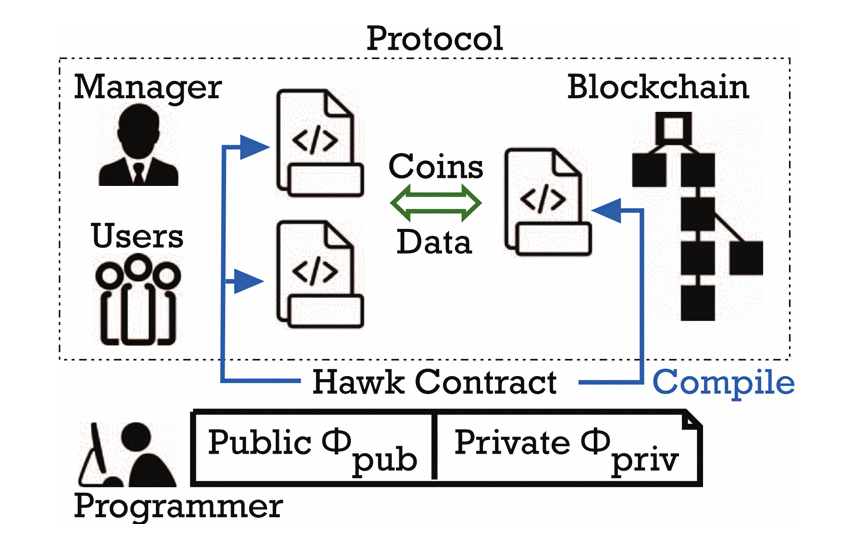
\includegraphics[width=.8\linewidth]{1}
    \caption{Hawk Overview}
    \label{fig1}
\end{figure}

\begin{enumerate}
    \item 私有部分表示为$\phi _{priv}$,它接收各方的输入数据(例如,“石头、纸、剪刀”游戏中的选择)以及货币单位(例如,拍卖中的出价)。$\phi _{priv}$执行计算以确定各方之间的支付分配。例如,在拍卖中,获胜者的出价归卖方所有,而其他人的出价则被退还。私有 \textbf{Hawk} 程序$\phi _{priv}$旨在保护参与者的数据和货币交换。 
    \item 公有部分表示为$\varphi  _{pub}$,$\varphi  _{pub}$不涉及私人数据或金钱。
\end{enumerate}

我们的编译器会将 \textbf{Hawk} 程序编译成以下部分,这些部分共同定义了用户、管理器和区块链之间的加密协议:

\begin{itemize}
    \item 由所有共识节点执行的区块链程序;
    \item 由用户执行的程序;
    \item 由称为管理者的特殊促进方执行的程序。(稍后将对其进行解释。)
\end{itemize}

\subsection{安全保障}

\textbf{Hawk} 的安全保障包括两个方面:

\begin{itemize}
    \item \textit{链上隐私}。链上隐私规定,交易隐私是针对公众(即,针对任何未参与合同的一方)提供的——除非合同方自己自愿披露信息。尽管在 \textbf{Hawk} 协议中,用户与区块链交换数据,并依靠它来确保公平性以防止中止,但在私有 \textbf{Hawk} 程序 $\phi _{priv}$ 中交易的资金流和金额以加密方式隐藏在公众的视野之外。非正式地,这是通过向区块链发送“加密”信息,并依靠零知识证明来强制执行合同的正确性和资金节约来实现的。
    \item \textit{合同保障}。虽然链上隐私保护合同方的隐私不受公众(即未参与金融合同的各方)的影响,但合同安全性保护同一合同协议中的各方相互之间。 \textbf{Hawk} 假设合同各方自私地行动以最大化他们自己的经济利益。特别是,它们可以任意偏离规定的协议,甚至提前中止。因此,合同安全是一个多方面的概念,不仅包括机密性和真实性的密码概念,还包括存在作弊和中止行为时的财务公平性。理解合同安全的最好方法是通过一个具体的例子。
\end{itemize}

\subsection{最低信任管理者}

\textbf{Hawk} 合同的执行由一个称为管理者(manager)的特殊方推进。管理者可以看到用户的输入,并且被信任不会泄露用户的私人数据。但是管理者不能等同于可信任的第三方,即使管理者可以任意偏离协议或者与某一方勾结,管理者也不能影响合同的正确性,如果管理者终止了协议,其可能会收到经济处罚,并且用户也会获得相应的补偿。

管理者也不需要被信任来维护基础货币的安全性或隐私(例如,它不能双花、膨胀货币或对用户进行去匿名化)。此外,如果多个合约实例同时运行,则每个合约都可能指定不同的管理器,并且损坏的管理器的影响仅限于该实例。 最后,管理者角色可以用英特尔 SGX 等可信计算硬件实例化,或者用用户自己之间的多方计算代替。

\subsection{术语}

在以太坊 \cite{ref57} 中,协议的区块链部分称为以太坊合约。但是,本文将 \textbf{Hawk} 程序定义的整个协议称为合约;区块链的程序是更大协议的组成部分。

\section{示例:密封式拍卖}

\subsection{示例程序}

图\ref{fig2}展示了一个 \textbf{Hawk} 程序,用于实施密封的次价拍卖,其中出价最高的人获胜,但支付的价格是次高价格。众所周知,在某些假设下,二级价格拍卖会激励真实的投标,\cite{ref55} 重要的是投标人在不知道其他人的投标的情况下提交投标。我们的示例拍卖程序包含一个私有部分 $\phi _{priv}$,它决定了中标者和要支付的价格; 和一个公共部分 $\varphi  _{pub}$,它依靠公共存款来保护投标人免受中止的管理者的伤害。

目前,我们假设一组投标人是先验的。

\begin{figure}
    \centering
    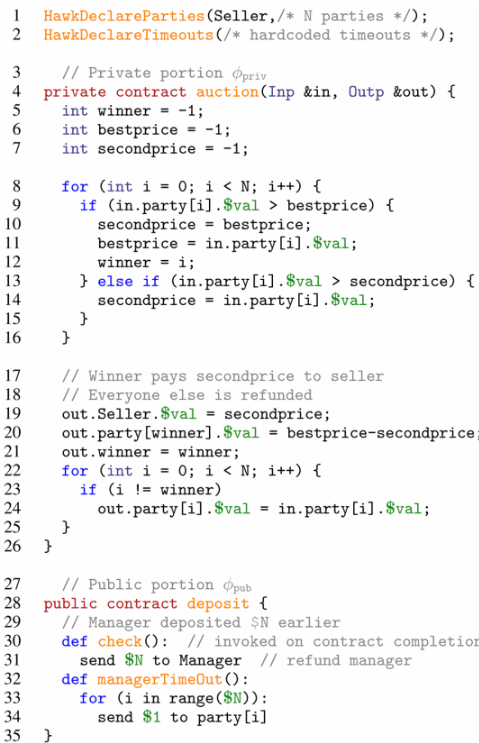
\includegraphics[width=.4\linewidth]{2}
    \caption{Hawk计划进行二价密封拍卖 \\ 本文中的代码描述在是我们实际实现的近似。}
    \label{fig2}
\end{figure}

\subsection{合约安全要求}

\textbf{Hawk} 将这个拍卖程序编译成加密协议。如之前所述,只要投标人和管理者不自愿披露信息,交易的隐私就会收到保护而不会公开。\textbf{Hawk} 还为合同方保证以下合同安全要求:

\begin{itemize}
    \item \textit{输入独立隐私}。每个用户在承诺自己的出价之前都不会看到其他人的出价(即使他们与潜在的恶意管理者勾结)。这样,用户的出价就独立于其他人的出价。
    \item \textit{后置隐私}。只要管理者不透露信息,即使在拍卖之后,用户的出价也会彼此(以及公众)保密。
    \item \textit{财产公平}。各方可能会试图过早退出合约,以避免付款或影响财富的重新分配。如果一方中止或拍卖管理者中止,则中止方将受到经济处罚,而其余各方将获得赔偿。正如密码学文献中众所周知的那样,这种公平性保证通常无法通过仅链外的协议(例如安全多方计算 \cite{ref7}\cite{ref17})来实现。 正如稍后解释的那样,\textbf{Hawk} 提供了内置机制,用于在特定超时后强制执行私人投标退款。 \textbf{Hawk} 还允许程序员定义其他规则,作为 \textbf{Hawk} 合同的一部分,以管理财务公平。
    \item \textit{对不诚实管理者的防范}。 我们确保针对不诚实的管理者的真实性:除了中止之外,不诚实的管理者不能影响拍卖的结果和资金的重新分配,即使它与一部分用户勾结。我们强调,为确保上述内容,输入独立隐私以防止有缺陷的管理者是先决条件。此外,如果管理者中止,则可能受到经济处罚,参与者获得相应的报酬。
\end{itemize}

具有上述安全和隐私要求的拍卖无法在现有的加密货币系统(如以太坊 \cite{ref57} 或 Zerocash \cite{ref11})上轻松实现。前者允许可编程性,但不保证交易隐私,而后者保证交易隐私,但其代价是可编程性甚至低于比特币。

\subsection{中止和超时机制}

使用超时处理中止。 如图 \ref{fig2} 所示的 \textbf{Hawk} 程序使用 \textsl{HawkDeclareTimeouts} 特殊语法声明超时参数。其声明了三个超时,其中 $T_1 < T_2 < T_3$:

$T_1$:\textbf{Hawk} 在$T_1$之后停止收集投标。

$T_2$: 所有用户都应在 $T_2$ 内向管理者开标;如果用户提交了投标但未能在 $T_2$ 之前打开,则其输入投标被视为 0(并且任何其他潜在输入数据被视为$\perp$ ),以便管理者可以继续。

$T_3$:如果管理者中止,用户可以在时间 $T_3$ 之后收回他们的私人投标。

公共 \textbf{Hawk} 合约 $\varphi  _{pub}$ 可以额外实施激励结构。 如果中止,我们的密封拍卖程序会重新分配经理的公开存款。 具体来说,在我们的密封拍卖程序中,$\varphi  _{pub}$ 定义了两个函数,即 check 和 managerTimeOut。 当 \textbf{Hawk} 合约在 $T_3$ 内完成执行时,将调用 check 函数,即 manager 没有中止。 否则,如果 \textbf{Hawk} 合约在 $T_3$ 内没有完成执行,就会调用 managerTimeOut 函数。 我们注意到,虽然没有明确写在代码中,但所有 \textbf{Hawk} 合约都有一个隐含的默认入口点来接受各方的存款——这些存款由合约扣留,直到它们被合约重新分配。投标人在提交投标前应检查管理人是否已公开存款。

\subsection{附加应用}

除了密封拍卖示例,\textbf{Hawk} 还支持各种其他应用程序。

\section{贡献}

据我们所知,\textbf{Hawk} 是第一个在去中心化加密货币系统中同时提供交易隐私和可编程性的系统。

\subsection{去中心化智能合约的正式模型}

我们是最早对区块链密码学模型进行正式学术处理的人之一。我们为密码学的区块链模型提出了一个正式的通用可组合性 (UC) 模型——这种形式模型具有独立的兴趣,通常可用于定义和建模区块链模型中协议的安全性。 Gyges 的工作 \cite{ref35} 也采用了我们的正式模型来设计犯罪智能合约。

在定义正式的区块链模型时,我们依靠称为包装器的概念来模块化我们的协议设计并简化表示。包装器在一个集中的地方处理一组常见的细节,例如计时器、假名、全局分类帐,这样它们就不需要在每个协议中重复。

\subsection{新密码学套件}

我们实现了一个新的加密套件,它将私人交易与可编程逻辑绑定在一起。我们的协议套件包含三个基本原语 freeze、compute 和 finalize。 freeze 原语允许各方不仅提交普通数据,而且还提交币。承诺的币在合约中被冻结,支付分配稍后将由程序 $\phi _{priv}$ 确定。 在计算过程中,各方向管理者开放他们承诺的数据和货币,以便管理者可以计算函数 $\phi _{priv}$。 根据 $\phi _{priv}$ 的结果,经理现在构造新的私人币以支付给每个接收者。 然后,经理向区块链提交新的私人币以及其良好格式的零知识证明。 此时,之前冻结的币现在在用户之间重新分配。 我们的协议套件严格概括了 Zerocash,因为 Zerocash 只实现了用户之间的私人资金转移,没有可编程性。

我们使用理想功能定义原语的安全性,并在基于模拟的范式下正式证明我们的结构的安全性。

\subsection{实施与评估}

我们构建了一个 \textbf{Hawk} 原型,并通过实施几个示例应用程序来评估它的性能,包括密封投标拍卖、“石头剪刀布”游戏、众筹应用程序和掉期金融工具。我们提出了有趣的协议优化,相对于简单的实现,我们的性能提高了 10 倍。 我们表明,对于大约 100 个参与方(例如,拍卖和众筹),经理的加密计算(协议中最昂贵的部分)使用 4 个内核不到 2.85 分钟,相当于不到 0.14 美元的 EC2 时间。此外,所有链上计算(由所有矿工执行)非常便宜,所有情况下都在 20 毫秒以下。 我们将在不久的将来开源我们的 \textbf{Hawk} 框架。

\section{背景及相关工作}

\subsection{背景}

最初的比特币通过既不是图灵完备也不是用户友好的脚本语言提供有限的可编程性。之前在比特币上创建类似智能合约的应用程序(例如,彩票 \cite{ref7}\cite{ref17}、小额支付\cite{ref4}、可验证计算 \cite{ref40})的许多努力已经证明了改造比特币脚本语言的难度——这很好地服务于激发图灵完备、用户友好的智能合约语言。

以太坊是第一个图灵完备的去中心化智能合约系统。随着以太坊即将推出,公司和爱好者已经在以太坊之上或通过分叉以太坊来构建大量智能合约应用程序,例如预测市场 \cite{ref3}、供应链来源 \cite{ref6}、基于众筹的筹款 \cite{ref1} 以及安全和衍生品交易 \cite{ref28}。

\textbf{区块链安全性}:
就像早期为加密货币设计智能合约应用程序的作品一样,我们依靠底层去中心化区块链来保证安全。因此,我们假设当对手没有使用大部分计算能力时,区块链的共识协议会获得安全性。 现有的加密货币设计具有启发式安全性。 一方面,研究人员已经确定了对系统各个方面的攻击 \cite{ref29}\cite{ref34};另一方面,正式理解区块链共识安全性的努力已经开始\cite{ref32}\cite{ref45}。

\textbf{最小化链上成本}:
由于每个矿工都会在验证每笔交易的同时执行智能合约程序,因此包括比特币和以太坊在内的加密货币会收取与执行成本大致相关的交易费用。虽然我们没有明确对此类费用进行建模,但我们设计我们的协议以通过在链下执行大部分重量级计算来最小化链上成本。

\subsection{附加相关工作}

\textbf{利用区块链实现财务公平}:
一些先前的工作已经探索了如何利用区块链技术来实现协议设计的公平性。 例如,本托夫等人 \cite{ref17},Andrychowicz 等人 \cite{ref7},Kumaresan 等人 \cite{ref40},Kiayias 等人 \cite{ref36},以及 Zyskind 等人 \cite{ref59}展示了如何使用比特币来确保安全多方计算协议的公平性。 这些协议还执行各种类型的链下安全计算,但不保证交易隐私(即隐藏货币流动和交易金额)。例如,尚不清楚如何使用这些早期技术来实现我们的密封拍卖示例。其次,这些早期的作品要么不提供系统实现,要么只为特定应用程序(例如彩票)提供实现。相比之下,\textbf{Hawk} 提供了一个通用平台,使非专业程序员可以轻松开发保护隐私的智能合约。

\textbf{智能合约}:
可编程电子“智能合约”的概念可以追溯到近二十年前\cite{ref53}。 除了最近保证真实性但不保证隐私的去中心化加密货币外,其他智能合约实现还依赖受信任的服务器来保证安全\cite{ref46}。因此,我们的工作最接近于实现各方与执行涉及金钱和数据的程序的可信赖“虚拟计算机”交互的最初愿景。

\textbf{密码学编程框架}:
一些工作已经开发了将高级程序作为规范并生成加密实现的编程框架,包括用于安全多方计算的编译器 \cite{ref19}\cite{ref39}\cite{ref41}\cite{ref51}、经过身份验证的数据结构 \cite{ref44} 和(零知识)证明\cite{ref12}\cite{ref30}\cite{ref31}\cite{ref49}等展示如何生成安全的分布式协议,例如密封拍卖、战舰游戏和银行应用程序 \cite{ref58}。 这些作品支持各种安全概念,但它们都没有直接与金钱交互或利用公共区块链来确保金融公平。因此,我们的工作是最早将“构造正确”密码学方法与智能合约相结合的工作之一。

\textbf{并行工作}:
我们的框架是第一个为比特币、以太坊和许多其他流行的去中心化加密货币所体现的去中心化区块链提供完整正式模型的框架。在并行和独立的工作中,Kiayias 等人。 \cite{ref36} 还在(通用)通用可组合性框架 \cite{ref23} 中提出了一个区块链模型,并使用它得出类似于我们在在线版本 \cite{ref37} 中描述的结果,即具有公共存款的公平 MPC。然而,其形式主义的“可编程性”仅限于其特定应用(即具有公共存款的公平 MPC)。相比之下,我们的形式主义设计目标更广泛,即便于协议设计者在区块链模型中设计丰富的协议类别。特别是,我们的现实世界包装器和理想世界包装器都模拟了任意用户定义的合同程序的存在,它们与双方和分类帐交互。 Gyges 的工作 \cite{ref35} 也采用了我们的形式主义,证明了它的广泛用途。

\chapter{密码学的区块链模型}

\section{区块链模型}

我们首先非正式地描述信任模型和假设。然后,我们为“密码学的区块链模型”提出了一个正式的框架,用于指定和推理协议的安全性。

在本文中,区块链是指一组分散的矿工,他们运行安全的共识协议以就全球状态达成一致。因此,我们将区块链视为概念上的可信方,其正确性和可用性值得信赖,但隐私方面不受信任。区块链不仅维护了一个全球账本,用于存储每个假名的余额,而且还执行用户定义的程序。更具体地说,我们做出以下假设:

\begin{itemize}
    \item \textit{时间}。区块链知道一个以轮次递增的离散时钟。我们可以互换使用轮数和历元这两个术语。
    \item \textit{公共状态}。各方都可以观察到区块链的状态。这意味着所有各方都可以观察区块链上的公共账本,以及任何用户区块链程序(合约协议的一部分)的状态。
    \item \textit{消息传递}。发送到区块链的消息将在下一轮开始时到达。网络攻击者可以任意重新排序在同一轮内发送到区块链的消息。这意味着对手可能会尝试进行抢先攻击(也称为密码学家的抢先对手),例如,在观察到诚实用户正在交易股票时,对手会通过发送交易相同股票的竞赛交易来抢占先机。尽管有这样的对抗性消息传递时间表,我们的协议仍应被证明是安全的。 

    我们假设所有各方都有一个可靠的区块链通道,并且对手不能丢弃一方发送到区块链的消息。实际上,这意味着覆盖网络必须有足够的冗余。但是,对手可以将各方之间传递的消息从区块链中删除。
    \item \textit{化名}。用户在与区块链通信时可以组成无限多项式的假名。
    \item \textit{正确性和可用性}。我们假设区块链将正确执行任何规定的计算。我们还假设区块链始终可用。
\end{itemize}

\subsection{通用区块链模型的优势}:

我们采用通用区块链模型,其中区块链可以运行任意图灵完备程序。相比之下,先前和同时进行的工作 \cite{ref7}\cite{ref17}\cite{ref40}\cite{ref50} 改进了比特币有限且难以使用的脚本语言的工件。 在第 7 节和在线版本 \cite{ref37} 中,我们提出了额外的理论结果,证明我们的通用区块链模型产生了渐近更有效的密码协议。

\section{正式区块链建模}

我们的论文采用了精心设计的符号系统,这样读者就可以在不了解我们形式建模的精确细节的情况下理解我们的结构。

然而,我们强调,我们给出了功能和安全性的正式、精确的规范,并且我们的协议在通用可组合性 (UC) 框架下被正式证明是安全的。在此过程中,我们做出了独立利益的单独贡献:我们是第一个提出正式的、基于 UC 的框架来描述和证明与区块链交互的分布式协议的安全性 - 我们将我们的正式模型称为“ 密码学的区块链模型”。

\subsection{程序、包装器和功能}

在本文的其余部分,我们将描述理想的规范,以及由区块链、用户和管理器分别作为用伪代码编写的程序执行的协议片段。我们将它们分别称为理想程序(记为 Ideal)、区块链程序(记为 B 或 Blockchain)和用户/管理者程序(记为 UserP)。

我们所有的伪代码风格程序在 UC 框架中都有精确的含义。为了将程序“编译”为 UC 风格的功能或协议,我们将包装器应用于程序。具体来说,我们定义了以下类型的包装器:

\begin{itemize}
    \item 理想包装器$\mathcal{F} ( \cdot )$将理想程序 IdeaP 转化为 UC 理想功能$\mathcal{F} ( IdeaP )$。
    \item 区块链包装器$\mathcal{G} ( \cdot )$将区块链程序 B 转化为区块链功能$\mathcal{G} ( B )$。区块链功能$\mathcal{G} ( B )$对在区块链上执行的程序进行建模。
    \item 协议包装器$\prod ( \cdot )$将用户/管理者程序 UserP 转换为用户端或者管理者端协议$\prod ( UserP )$。
\end{itemize}

使用包装器的一个重要原因是,包装器实现了每个智能合约应用程序所需的一组通用特性,包括时间、公共分类账、假名和消息的对抗性重新排序——这样,我们不需要为每个区块链应用程序重复这个符号。

\section{编写程序的约定}

我们基于包装器的系统将符号模块化,并允许我们使用一组简单的约定来编写用户定义的理想程序、区块链程序和用户协议。我们将在下面描述这些约定。

\subsection{定时器激活点}

计时器激活点理想的功能包装器 $\mathcal{F} ( \cdot )$ 和区块链包装器 $\mathcal{G} ( \cdot )$ 实现了一个循环前进的时钟。 每次时钟提前,包装器都会调用 Timer 激活点。 因此,按照惯例,我们允许理想程序或区块链程序可以定义一个 Timer 激活点。 Timer 激活点下可以实现超时操作(例如,一定超时后退款)。

\subsection{理想程序中的延迟处理}

在编写区块链程序时,由于 $\mathcal{G} ( \cdot )$ 包装器,区块链程序接收到的每条消息都已经延迟了一轮。

在编写理想程序时,我们引入了一个简单的约定来表示延迟计算。以灰色背景编写的程序指令表示计算不会立即发生,而是推迟到下一次计时器点击的开始。这是一种方便的简写,因为在我们的现实世界协议中,实际上由区块链功能完成的任何计算都会被延迟。例如,在我们的 IdealPcash 理想程序中(参见图\ref{fig3}),每当理想功能收到铸币或倒酒消息时,都会立即通知理想对手 S;但是,消息的处理会延迟到下一次计时器点击。形式上,延迟处理可以简单地通过存储状态并在下次定时器点击时调用延迟的程序指令来实现。按照惯例,我们假设延迟指令在 Timer 调用开始时被调用。换句话说,在下一次定时器点击时,延迟的指令首先被执行。

\begin{figure}
    \centering
    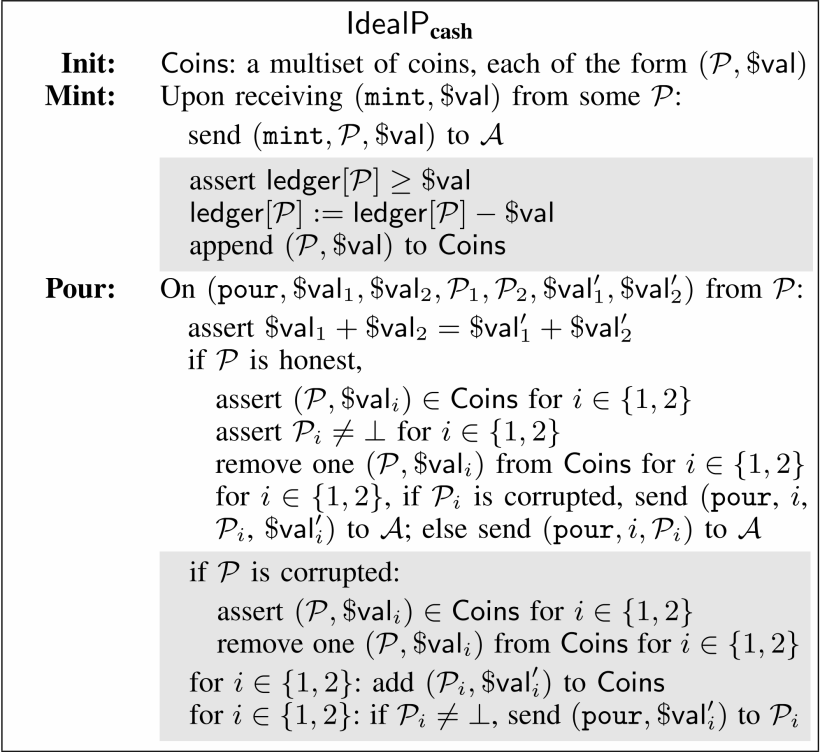
\includegraphics[width=.8\linewidth]{3}
    \caption{$IdealP_{cash}$ 的定义}
    \label{fig3}
\end{figure}

\subsection{化名}

理想程序、区块链程序、用户端程序中出现的所有当事人标识,默认都是指假名。 当我们写“收到来自某个 P 的消息时”时,它接受来自任何假名的消息。 每当我们写“从 P 接收消息时”,没有关键字 some 时,它接受来自固定笔名 P 的消息,通常我们指的是哪个笔名从上下文中是清楚的。

每当我们在用户程序中写“send m to $\mathcal{G} ( B )$ as nym P”时,都会向协议包装器 Π 发送一条内部消息(“send”,m,P)。 然后,协议包装器将使用假名 P 适当地验证消息。

当上下文清楚时,我们避免写成“as nym P”,而简单地写成“send m to $\mathcal{G} ( B )$”。我们的正式系统还允许用户匿名向区块链发送消息——尽管本文不会使用此选项。

\subsection{帐本和汇款}

在我们的理想程序和区块链程序中,公共分类账被称为分类账。 当一方将 \$amt 发送到理想程序或区块链程序时,这代表了普通的消息传输。 只有当理想程序或区块链程序更新公共分类账本时,才会发生资金转移。 换句话说,符号\$只是为了可读性(区分与货币相关的变量和其他变量)而采用的,并没有特殊的含义或意义。 可以简单地将这个变量视为具有货币类型。

\chapter{密码学抽象}

我们现在以理想程序的形式描述我们的密码学抽象。理想的程序定义了我们希望通过编写规范来实现的正确性和安全性要求,并假设存在完全受信任的一方。我们稍后将证明我们的现实世界协议(基于智能合约)可以安全地模拟理想程序。如前所述,理想的程序必须与包装器 $\mathcal{F}$ 相结合才能被赋予精确的执行语义。

% 参考文献
\begin{thebibliography}{99}  
    \bibitem{ref1} [online] Available: http://koinify.com.
    \bibitem{ref2} Amazon ec2 pricing, [online] Available: http://aws.amazon.com/ec2/pricing/.
    \bibitem{ref3} Augur, [online] Available: http://www.augur.net/.
    \bibitem{ref4} bitoinj, [online] Available: https://bitcoinj.github.io/.
    \bibitem{ref5} "The rise and rise of bitcoin", Documentary.
    \bibitem{ref6} Skuchain, [online] Available: http://www.skuchain.com/.
    \bibitem{ref7} M. Andrychowicz, S. Dziembowski, D. Malinowski and L. Mazurek, "Secure Multiparty Computations on Bitcoin", S\&P, 2013.
    \bibitem{ref8} G. Asharov, A. Beimel, N. Makriyannis and E. Omri, "Complete characterization of fairness in secure two-party computation of boolean functions", TCC, 2015.
    \bibitem{ref9} M. Bagnoli and B. L. Lipman, "Provision of public goods: Fully implementing the core through private contributions", The Review of Economic Studies, 1989.
    \bibitem{ref10} R. Beaulieu, D. Shors, J. Smith, S. Treatman-Clark, B. Weeks and L. Wingers, The simon and speck families of lightweight block ciphers, [online] Available: http://ia.cr/2013/404.
    \bibitem{ref11} E. Ben-Sasson, A. Chiesa, C. Garman, M. Green, I. Miers, E. Tromer, et al., "Zerocash: Decentralized anonymous payments from Bitcoin", S\&P, 2014.
    \bibitem{ref12} E. Ben-Sasson, A. Chiesa, D. Genkin, E. Tromer and M. Virza, "Snarks for C: verifying program executions succinctly and in zero knowledge", CRYPTO, 2013.
    \bibitem{ref13} E. Ben-Sasson, A. Chiesa, M. Green, E. Tromer and M. Virza, "Secure sampling of public parameters for succinct zero knowledge proofs", S\&P, 2015.
    \bibitem{ref14} E. Ben-Sasson, A. Chiesa, E. Tromer and M. Virza, "Scalable zero knowledge via cycles of elliptic curves", CRYPTO, 2014.
    \bibitem{ref15} E. Ben-Sasson, A. Chiesa, E. Tromer and M. Virza, "Succinct noninteractive zero knowledge for a von neumann architecture", Security, 2014.
    \bibitem{ref16} E. Ben-Sasson and M. Sudan, "Short pcps with polylog query complexity", SIAM J. Comput., 2008.
    \bibitem{ref17} I. Bentov and R. Kumaresan, "How to Use Bitcoin to Design Fair Protocols", CRYPTO, 2014.
    \bibitem{ref18} N. Bitansky, R. Canetti, A. Chiesa and E. Tromer, "Recursive composition and bootstrapping for snarks and proof-carrying data", STOC, 2013.
    \bibitem{ref19} D. Bogdanov, S. Laur and J. Willemson, "Sharemind: A Framework for Fast Privacy-Preserving Computations", ESORICS, 2008.
    \bibitem{ref20} J. Bonneau, A. Miller, J. Clark, A. Narayanan, J. A. Kroll and E. W. Felten, "Research Perspectives and Challenges for Bitcoin and Cryptocurrencies", S\&P, 2015.
    \bibitem{ref21} R. Canetti, "Universally composable security: A new paradigm for cryptographic protocols", FOCS, 2001.
    \bibitem{ref22} R. Canetti, "Universally composable signature certification and authentication", CSF, 2004.
    \bibitem{ref23} R. Canetti, Y. Dodis, R. Pass and S. Walfish, "Universally composable security with global setup", TCC, 2007.
    \bibitem{ref24} R. Cleve, "Limits on the security of coin flips when half the processors are faulty", STOC, 1986.
    \bibitem{ref25} C. Costello, C. Fournet, J. Howell, M. Kohlweiss, B. Kreuter, M. Naehrig, et al., "Geppetto: Versatile verifiable computation", S \& P, 2015.
    \bibitem{ref26} G. Danezis, C. Fournet, M. Kohlweiss and B. Parno, "Pinocchio Coin: building Zerocoin from a succinct pairing-based proof system", PETShop, 2013.
    \bibitem{ref27} C. Decker and R. Wattenhofer, "Bitcoin transaction malleability and mtgox" in ESORICS, Springer, 2014.
    \bibitem{ref28} A. K. R. Dermody and O. Slama, Counterparty announcement, [online] Available: https://bitcointalk.org/index.php?topic=395761.0.
    \bibitem{ref29} I. Eyal and E. G. Sirer, "Majority is not enough: Bitcoin mining is vulnerable", FC, 2014.
    \bibitem{ref30} C. Fournet, M. Kohlweiss, G. Danezis and Z. Luo, "Zql: A compiler for privacy-preserving data processing", USENIX Security, 2013.
    \bibitem{ref31} M. Fredrikson and B. Livshits, "Zø: An optimizing distributing zero-knowledge compiler", USENIX Security, 2014.
    \bibitem{ref32} J. A. Garay, A. Kiayias and N. Leonardos, "The bitcoin backbone protocol: Analysis and applications", Eurocrypt, 2015.
    \bibitem{ref33} R. Gennaro, C. Gentry, B. Parno and M. Raykova, "Quadratic span programs and succinct NIZKs without PCPs", Eurocrypt, 2013.
    \bibitem{ref34} E. Heilman, A. Kendler, A. Zohar and S. Goldberg, "Eclipse attacks on bitcoin's peer-to-peer network", USENIX Security, 2015.
    \bibitem{ref35} A. Juels, A. Kosba and E. Shi, "The ring of gyges: Using smart contracts for crime", Manuscript, 2015.
    \bibitem{ref36} A. Kiayias, H.-S. Zhou and V. Zikas, Fair and robust multi-party computation using a global transaction ledger, [online] Available: http://ia.cr/2015/574.
    \bibitem{ref37} A. Kosba, A. Miller, E. Shi, Z. Wen and C. Papamanthou, Hawk: The blockchain model of cryptography and privacy-preserving smart contracts, [online] Available: http://ia.cr/2015/675.
    \bibitem{ref38} A. Kosba, Z. Zhao, A. Miller, H. Chan, C. Papamanthou, R. Pass, et al., How to use snarks in universally composable protocols, 2015, [online] Available: https://eprint.iacr.org/2015/1093.
    \bibitem{ref39} B. Kreuter, B. Mood, A. Shelat and K. Butler, "PCF: A portable circuit format for scalable two-party secure computation", Security, 2013.
    \bibitem{ref40} R. Kumaresan and I. Bentov, "How to Use Bitcoin to Incentivize Correct Computations", CCS, 2014.
    \bibitem{ref41} C. Liu, X. S. Wang, K. Nayak, Y. Huang and E. Shi, "ObliVM: A programming framework for secure computation", S\&P, 2015.
    \bibitem{ref42} S. Meiklejohn, M. Pomarole, G. Jordan, K. Levchenko, D. McCoy, G. M. Voelker, et al., "A fistful of bitcoins: characterizing payments among men with no names", IMC, 2013.
    \bibitem{ref43} I. Miers, C. Garman, M. Green and A. D. Rubin, "Zerocoin: Anonymous Distributed E-Cash from Bitcoin", S\&P, 2013.
    \bibitem{ref44} A. Miller, M. Hicks, J. Katz and E. Shi, "Authenticated data structures generically", POPL, 2014.
    \bibitem{ref45} A. Miller and J. J. LaViola, "Anonymous Byzantine Consensus from Moderately-Hard Puzzles: A Model for Bitcoin", 2014.
    \bibitem{ref46} M. S. Miller, C. Morningstar and B. Frantz, "Capability-based financial instruments", FC, 2001.
    \bibitem{ref47} N. Mouha, B. Mennink, A. Van, D. Watanabe, B. Preneel and I. Verbauwhede, "Chaskey: An efficient mac algorithm for 32-bit microcontrollers" in Selected Areas in Cryptography-SAC 2014, Springer, pp. 306-323, 2014.
    \bibitem{ref48} S. Nakamoto, Bitcoin: A Peer-to-Peer Electronic Cash System, 2009, [online] Available: http://bitcoin.org/bitcoin.pdf.
    \bibitem{ref49} B. Parno, C. Gentry, J. Howell and M. Raykova, "Pinocchio: Nearly practical verifiable computation", S\&P, 2013.
    \bibitem{ref50} R. Pass and Abhi Shelat, "Micropayments for peer-to-peer currencies", CCS, 2015.
    \bibitem{ref51} A. Rastogi, M. A. Hammer and M. Hicks, "Wysteria: A programming language for generic mixed-mode multiparty computations", S\&P, 2014.
    \bibitem{ref52} D. Ron and A. Shamir, "Quantitative Analysis of the Full Bitcoin Transaction Graph", FC, 2013.
    \bibitem{ref53} N. Szabo, "Formalizing and securing relationships on public networks", 1997.
    \bibitem{ref54} N. van Saberhagen, Cryptonote v 2.0, 2013, [online] Available: https://goo.gl/kfojVZ.
    \bibitem{ref55} W. Vickrey, "Counterspeculation auctions and competitive sealed tenders", Journal of finance, 1961.
    \bibitem{ref56} R. S. Wahby, S. T. V. Setty, Z. Ren, A. J. Blumberg and M. Walfish, "Efficient RAM and control flow in verifiable outsourced computation", NDSS, 2015.
    \bibitem{ref57} G. Wood, Ethereum: A secure decentralized transaction ledger, [online] Available: http://gavwood.com/paper.pdf.
    \bibitem{ref58} L. Zheng, S. Chong, A. C. Myers and S. Zdancewic, "Using replication and partitioning to build secure distributed systems", S\&P, 2003.
    \bibitem{ref59} G. Zyskind, O. Nathan and A. Pentland, Enigma: Decentralized computation platform with guaranteed privacy.
\end{thebibliography}
\backmatter
\end{document}